\index{Linear time-invariant systems}{Linear time-invariant systems}
(LTI) are an important class of systems that can be analyzed easily in frequency domain. An LTI system is equivalent to \emph{\index{convolution}{convolution}} of the \emph{impulse response} of the system. 
The focus of this chapter is to learn more about what these concepts are. 

\section{Example: Running average filter}
Here's an example of a discrete-time system that you might use to smooth a noisy signal:
\begin{equation}
  y[n] = \frac{1}{15}\sum_{k=-7}^{7} x[n-k]\,\,.
  \label{eq:running_mean}
\end{equation}
What does this system do? It averages together 15 neighboring values of input signal $x[n]$. Figure \ref{fig:avg_filter} shows a demonstration of this system in action. 
The blue line indicates a noisy input signal $x[n]$, and the orange line depicts the output $y[n]$ of the running mean filter given in Equation \ref{eq:running_mean}. 
As you might expect, the output of the system is a smoother version of the input signal.
\begin{figure}
  \begin{center}
    \includegraphics[width=\textwidth]{code/016_smoothing/smoothing.png}
  \end{center}
  \caption{A running average filter is often used to smooth a noisy
    signal. You can find the Python code used to produce this example
    in \texttt{016\_smoothing/smoothing.py}.}
  \label{fig:avg_filter}
\end{figure}

\section{Finite impulse response filter}
\begin{marginfigure}

\begin{center}
  \begin{tikzpicture}[node distance=3cm,auto,>=latex']
    \node [int] (a) {LTI};
    \node (b) [left of=a, coordinate] {a};
%    \node (c) [below=a,node distance=3cm] {a};

%\node [int, pin={[init]above:$p_0$}] (c) [right of=a] {$\frac{1}{s}$};
    \node [coordinate] (end) [right of=a]{};
    \path[->] (b) edge node {$x[n]$} (a);
    \path[->] (b) edge node [below]{$\delta[n]$} (a);

%\path[->] (a) edge node {$v$} (c);
    \draw[->] (a) edge node {$y[n]$} (end) ;
    \draw[->] (a) edge node [below]{$h[n]$} (end) ;

\end{tikzpicture}
\end{center}
\caption{Discrete-time LTI systems are characterized by an impulse response $h[n]$, which is the response of the LTI system to a unit impulse signal.}
\end{marginfigure}

The previous system shown in Equation \ref{eq:running_mean} is a special case of a more general type of discrete-time LTI system, 
known as a Finite Impulse Response (FIR) filter. This type of signal is often used in digital signal processing. 
An FIR filter is defined as follows:
\begin{equation}
  \boxed{
    y[n] = \sum_{k=-M}^{N} b_k x[n-k]\,\,.
  }
  \label{eq:fir_filter}
\end{equation}
The coefficients $b_k \in \mathbb{C}$ here are constant valued coefficients. As the name implies, there is a finite number of non-zero coefficients $b_k$. 
In the case of the running average filter in Equation \ref{eq:running_mean}, there would be 15 coefficients, which are all $b_k=1/15$.

\section{General discrete-time LTI system}
What if we allow there to be infinitely many coefficients for the system given in Equation \ref{eq:fir_filter}? We get the following:
\begin{equation}
    y[n] = \sum_{k=-\infty}^{\infty} b_k x[n-k] = \sum_{k=-\infty}^{\infty} b[k] x[n-k]\,\,.
\end{equation}
This turns out to be the general representation for arbitrary discrete-time LTI systems! In this case, it makes sense to think of the infinitely many coefficients $b_k$ as a signal $b[k]$.

For discrete-time LTI systems in general, the output of a system is given by a discrete-time convolution sum of the input signal $x[n]$ with an impulse response $h[n]$:

\begin{marginfigure}
  \begin{center}
          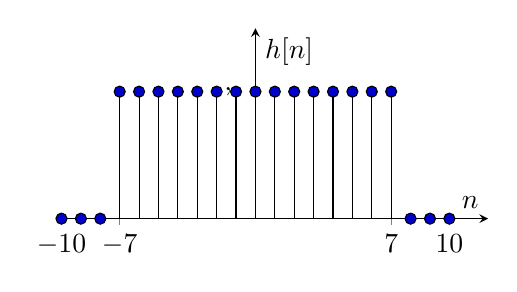
\begin{tikzpicture}
          \begin{axis}[width=7cm,height=4cm,ymin=0,xmin=-10,ymax=0.1,xmax=12,
         xtick={-10,-7,0,7,10},
              ytick={0,1,2,3},
              ytick={0,0.0667},
              yticklabel={,,},
          ylabel={$h[n]$},
      xlabel={$n$}, axis lines = center]
     \addplot+[ycomb,color=black] plot coordinates {(-10,0)(-9,0)(-8,0)(-7,0.0667)(-6,0.0667)(-5,0.0667)(-4,0.0667)(-3,0.0667)(-2,0.0667)(-1,0.0667)(0,0.0667)(1,0.0667)(2,0.0667)(3,0.0667)(4,0.0667)(5,0.0667)(6,0.0667)(7,0.0667)(8,0)(9,0)(10,0)};
  \end{axis}
  \end{tikzpicture}
  \end{center}
  \caption{The impulse response of the 15 point running mean filter described in Equation \ref{eq:running_mean}.}
\end{marginfigure}

\begin{equation}
  \boxed{
    y[n] = \mathcal{T}\{x[n]\}=\sum_{k=-\infty}^{\infty} h[k] x[n-k]\,\,.
  }
  \label{eq:conv_dlti}
\end{equation}
The impulse response is defined as follows:
\begin{equation}
  \boxed{
    h[n] = \mathcal{T}\{\delta[n]\}\,\,.
  \label{eq:conv_ireq}    
    }
\end{equation}
It is hopefully easy to see that Equation \ref{eq:conv_dlti} is valid for all LTI systems. %This was already briefly discussed earlier in the chapter on Fourier transforms.

A linear system $\mathcal{T}\{\cdot\}$\footnote{If linearity applies for two input signals $\mathcal{T}\{\alpha_1 s_1[n] + \alpha_2 s_2[n]\} = \alpha_1 \mathcal{T}\{s_1[n]\}+\alpha_2 \mathcal{T}\{s_2[n]\}$, it also applies for linear combinations of three or more signals.} must by definition satisfy the following relation:
\begin{equation}
  \mathcal{T}\left\{\sum_{k=-\infty}^{\infty} \alpha_k s_k[n]\right\} = \sum_{k=-\infty}^{\infty} \alpha_k \mathcal{T}\{s_k[n]\}\,\,.
  \label{eq:linearity_gen}
\end{equation}
Here $\alpha_k \in \mathbb{C}$ are arbitrary constants and $s_k[n]$ are arbitrary signals.

Time-invariance of $\mathcal{T}\{\cdot\}$, on the other hand, implies that for any time shift $k$ in the input, the output is correspondingly time shifted. 
This is valid for any input signal $x[n]$:
\begin{equation}
y[n-k] = \mathcal{T}\{x[n-k]\}\,\,,
\end{equation}
if 
\begin{equation}
y[n]=\mathcal{T}\{x[n]\}\,\,.
\end{equation}
It is possible to represent any signal $x[n]$ with the help of time-shifted unit impulse signals\sidenote{Recall that the discrete-time unit impulse is defined as: 
\begin{equation}
\delta[n] = \left\{
  \begin{array}{rcr}
    1 & \mathrm{when} & n=0 \\
    0 & \mathrm{otherwise} & \\
  \end{array}
\right.\,\,.
\end{equation}

It is the discrete-time equivalent of a Dirac delta function. The unit impulse is shown in Figure \ref{fig:dt_unit_impulse}.
}:
\begin{equation}
  x[n] = \sum_{k=-\infty}^{\infty} x[k]\delta[n-k]\,\,.
\end{equation}
Linearity implies that:
\begin{equation}
\mathcal{T}\{x[n]\} = \mathcal{T}\left\{\sum_{k=-\infty}^{\infty}x[k]\delta[n-k]\right\} = \sum_{k=-\infty}^{\infty}x[k] \mathcal{T}\{\delta[n-k]\}\,\,.
\end{equation}
\if 0
\begin{marginfigure}
\begin{center}
    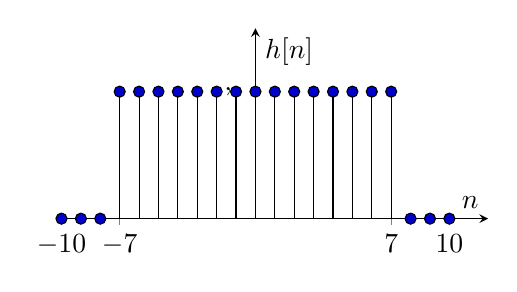
\begin{tikzpicture}
      \begin{axis}[width=7cm,height=4cm,ymin=0,xmin=-10,ymax=0.1,xmax=12,
                   xtick={-10,-7,0,7,10},
                  ytick={0,1,2,3},
             ytick={0,0.0667},
             yticklabel={,,},
             ylabel={$h[n]$},
             xlabel={$n$}, axis lines = center]
        \addplot+[ycomb,color=black] plot coordinates {(-10,0)(-9,0)(-8,0)(-7,0.0667)(-6,0.0667)(-5,0.0667)(-4,0.0667)(-3,0.0667)(-2,0.0667)(-1,0.0667)(0,0.0667)(1,0.0667)(2,0.0667)(3,0.0667)(4,0.0667)(5,0.0667)(6,0.0667)(7,0.0667)(8,0)(9,0)(10,0)};
      \end{axis}
     \end{tikzpicture}
\end{center}
\caption{The impulse response of the 15 point running mean filter described in Equation \ref{eq:running_mean}.}
\end{marginfigure}
\fi
\noindent The equation above is the same as Equation \ref{eq:linearity_gen} with $s_k[n] = \delta[n-k]$ and $\alpha_k=x[k]$.  Due to time-invariance,
we can relate the impulse response $h[n]$ delayed by $k$ to the term
on the right-hand side above. If a unit impulse fed into the system is
\begin{equation}
h[n] = \mathcal{T}\{\delta[n]\},
\end{equation}
\begin{marginfigure}
  \begin{center}
    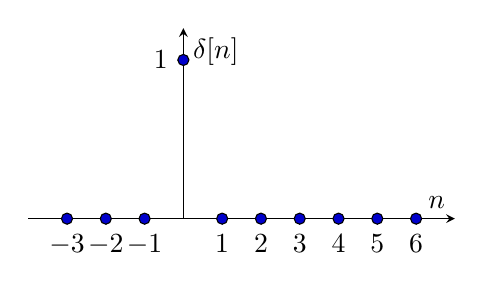
\begin{tikzpicture}
      \begin{axis}[width=7cm,height=4cm,ymin=0,xmin=-4,ymax=1.2,xmax=7,
                   xtick={-3,-2,-1,0,1,2,3,4,5,6},
                   ytick={0,1,2,3},
                   ylabel={$\delta[n]$},
                   xlabel={$n$}, axis lines = center]
          \addplot+[ycomb,color=black] plot coordinates {(-3,0) (-2,0) (-1,0) (0,1) (1,0) (2,0) (3,0) (4,0) (5,0) (6,0)};
      \end{axis}
     \end{tikzpicture}
     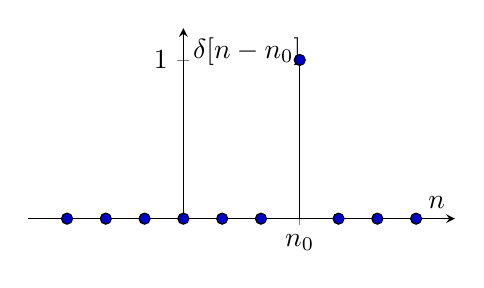
\begin{tikzpicture}
        \begin{axis}[width=7cm,height=4cm,ymin=0,xmin=-4,ymax=1.2,xmax=7,
          xtick={3},
          xticklabels={$n_0$},
          ytick={0,1,2,3},
          ylabel={$\delta[n-n_0]$},
          xlabel={$n$}, axis lines = center]
          \addplot+[ycomb,color=black] plot coordinates {(-3,0) (-2,0) (-1,0) (0,0) (1,0) (2,0) (3,1) (4,0) (5,0) (6,0)};
        \end{axis}
      \end{tikzpicture}
  \end{center}
  \caption{Discrete-time unit impulse signal $\delta[n]$ and a time-shifted version $\delta[n-n_0]$ centered at $n=n_0$.}
  \label{fig:dt_unit_impulse}
\end{marginfigure}
then a time-shifted unit impulse corresponds to a time-shifted output:
\begin{equation}
h[n-k] = \mathcal{T}\{\delta[n-k]\}\,\,.
\end{equation}
Therefore, the output of an LTI system for an arbitrary input signal
$x[n]$ can be expressed using the impulse response $h[n]$ as follows:
\begin{equation}
  y[n] = \sum_{k=-\infty}^{\infty} x[k]h[n-k].
  \label{eq:convolution_intro}
\end{equation}
This type of equation is known as a discrete-time convolution sum. We have now shown that any discrete-time LTI system can be represented with such a convolution sum. 
Note that Equation \ref{eq:convolution_intro} isn't quite yet the same as Equation \ref{eq:conv_dlti}. We will later show in Equation \ref{eq:commutative_convolution_proof} that the convolution sum is commutative, i.e., that
\begin{equation}
 \sum_{k=-\infty}^{\infty} x[k]h[n-k] = \sum_{k=-\infty}^{\infty} h[k]x[n-k].
\end{equation}
Which completes the proof.

\subsection{Example: Impulse response of an FIR filter}
An FIR filter (Equation \ref{eq:fir_filter}) has the following impulse response:
\begin{equation}
h[n] = \sum_{k=-M}^{N} b_k \delta[n-k]\,\,.
\end{equation}
The signal $h[n]$ contains the values of the filter coefficients $h[n]=b_n$. Since there are a finite number of coefficients $b_k$, the impulse response $h[n]$ 
has non-zero values only in a finite range of samples. This is also where the name ``finite impulse response'' comes from.
\begin{marginfigure}
\begin{center}
  \begin{tikzpicture}[node distance=2cm,auto,>=latex']
    \node [int] (a) {FIR filter ($b_k$)};
    \node (b) [left of=a, coordinate] {a};
%    \node (c) [below=a,node distance=3cm] {a};

%\node [int, pin={[init]above:$p_0$}] (c) [right of=a] {$\frac{1}{s}$};
    \node [coordinate] (end) [right of=a]{};
    \path[->] (b) edge node {$\delta[n]$} (a);
    %\path[->] (a) edge node {$v$} (c);
    \draw[->] (a) edge node {$h[n]$} (end) ;
\end{tikzpicture}
\end{center}
\caption{The impulse response of an FIR filter is a signal that contains the coefficients. For a finite number of coefficients $b_k$, the length of 
the non-zero portion of the impulse response is finite, and hence the name FIR.}
\end{marginfigure}


\section{Impulse response}
Linear time-invariant (LTI) systems are fully characterized by an \index{impulse response} impulse response $h(t)$. 
This impulse response is obtained by feeding a unit impulse into the LTI system:
\begin{equation}
\boxed{
h(t) = \mathcal{T}\{\delta(t)\}\,\,.
}
\end{equation}
Using an impulse response, it is possible to represent the output of any LTI system as a convolution between the impulse response and the input signal.
\begin{equation}
\boxed{
y(t) = \mathcal{T}\{x(t)\} = h(t)*x(t) = \int_{-\infty}^{\infty} h(\tau)x(t-\tau)d\tau\,\,.
}
\end{equation}
Let's prove this. We'll first need to represent an arbitrary signal as a sum of unit impulses:
\begin{equation}
x(t)  = \int_{-\infty}^{\infty} x(\tau) \delta(t-\tau) d\tau\,\,.
\end{equation}
One way to think of this integral is that the unit impulse $\delta(t-\tau)$ ``selects'' the value of $x(\tau)$ where $\tau=t$. 
Another way to think of this is that the Dirac delta functions form a set of basis functions for representing the signal $x(t)$.

\tikzstyle{int}=[draw, minimum size=2em]
\tikzstyle{init} = [pin edge={to-,thin,black}]

\begin{marginfigure}
\begin{center}

  \begin{tikzpicture}[node distance=3cm,auto,>=latex']

    \node [int] (a) [align=center]{LTI };
    \node (b) [left of=a, coordinate] {a};
%    \node (c) [below=a,node distance=3cm] {a};

%\node [int, pin={[init]above:$p_0$}] (c) [right of=a] {$\frac{1}{s}$};
    \node [coordinate] (end) [right of=a]{};
    \path[->] (b) edge node {$\delta(t)$} (a);
  %  \path[->] (b) edge node [below]{$\delta(t)$} (a);

%\path[->] (a) edge node {$v$} (c);
    \draw[->] (a) edge node {$h(t)$} (end) ;
 %   \draw[->] (a) edge node [below]{$h(t)$} (end) ;

\end{tikzpicture}

\end{center}
\caption{A linear time-invariant system is characterized by an impulse response.}
\end{marginfigure}

You may recall that linearity of the system $\mathcal{T}\{\cdot\}$ implies that:
\begin{equation}
\mathcal{T}\{c_1 \delta(t-\tau_1) + c_2 \delta(t-\tau_2)\} = c_1 \mathcal{T}\{\delta(t-\tau_1)\}+ c_2 \mathcal{T}\{\delta(t-\tau_2)\}\,\,.
\end{equation}
Here I've used $\delta(t-\tau_1)$ and $\delta(t-\tau_2)$ as two different input signals. The terms $c_1,c_2\in \mathbb{C}$ are arbitrary complex valued constants.

Linearity must therefore also apply for the linear combination of an arbitrary number of inputs:
\begin{equation}
\mathcal{T}\left\{\sum_n x_n \delta(t-\tau_n)\right\} = \sum_n x_n \mathcal{T}\{\delta(t-\tau_n)\}\,\,.
\end{equation}
Linearity can be extended even further into a continuous linear combination:
\begin{equation}
\mathcal{T}\left\{\int_{-\infty}^{\infty} x(\tau)\delta(t-\tau)d\tau\right\} = \int_{-\infty}^{\infty} x(\tau) \mathcal{T}\{\delta(t-\tau)\} d\tau\,\,.
\end{equation}
We can simplify the right-hand side and get:
\begin{equation}
\int_{-\infty}^{\infty} x(\tau) \mathcal{T}\{\delta(t-\tau)\} d\tau = \mathcal{T}\left\{x(t)\right\}\,\,.
\end{equation}
In order to simplify the left-hand side, we have to rely on the property of \emph{time-invariance}. That is:
\begin{equation}
h(t) = \mathcal{T}\{\delta(t)\} \Rightarrow h(t-\tau) = \mathcal{T}\{\delta(t-\tau)\}\,\,.
\end{equation}
This now completes our proof:
\begin{equation}
y(t)=\int_{-\infty}^{\infty} x(\tau) h(t-\tau) d\tau = \mathcal{T}\left\{x(t)\right\}\qed\,\,.
\end{equation}
The output of a linear time-invariant system $y(t)=\mathcal{T}\{x(t)\}$ is a convolution of the system's 
impulse response $h(t)=\mathcal{T}\{\delta(t)\}$ with the input signal $x(t)$ fed into the system.

\section{Frequency response}
It is possible to view an LTI system as a filter, which modifies each frequency component of the input signal. 
How each frequency component of the input signal is modified, is determined by the Fourier 
transform of the impulse response of the LTI system, which we will call \index{frequency response} frequency response $\Hiw$.

Recall that every LTI system is characterized by an impulse response:
\begin{equation}
h(t) = \mathcal{T}\{\delta(t)\}\,\,.
\end{equation}
We also know that the output of the LTI system is a convolution between the input signal $x(t)$ and the impulse response, 
which is a multiplication in frequency domain:
\begin{equation}
y(t) = h(t)*x(t) \xleftrightarrow{\mathcal{F}} \hat{y}(\omega) = \Hiw \hat{x}(\omega)\,\,.
\end{equation}
The frequency response is therefore the Fourier transform of the impulse response of the LTI system:
\begin{equation}
\boxed{
\Hiw = \int_{-\infty}^{\infty} h(\tau)e^{-i\omega \tau}  d\tau\,\,.
}
\end{equation}
The absolute value $|\Hiw|$ is called the \index{magnitude response} magnitude response, and the phase angle $\angle \Hiw$ is 
called the \index{phase response} phase response. These determine how the LTI system modifies 
the amplitude and phase of each spectral component of the signal.

\newpage
\section{Convolution}

A convolution operation is defined for both continuous-time and
discrete-time signals. As we just saw, a convolution operation can be
interpreted as an LTI system applied to a signal.

The continuous-time convolution is defined as an integral:
\begin{equation}
\boxed{
  a(t)*b(t) = \int_{-\infty}^{\infty}a(\tau)b(t-\tau)d\tau\,\,.
}
\end{equation}
The discrete-time convolution is defined as a sum:
\begin{equation}
\boxed{
  a[n]*b[n] = \sum_{k=-\infty}^{\infty}a[k]b[n-k]\,\,.
}
\end{equation}

\section{Properties of a convolution}

The unit impulse is \emph{identity}:
\begin{equation}
  \boxed{
    a[n] = a[n]*\delta[n]\,\,.
    } 
\end{equation}
Convolution is \emph{commutative}:
\begin{equation}
  \boxed{
    a[n]*b[n] = b[n]*a[n]\,\,,
    }
\end{equation}
\emph{associative}:
\begin{equation}
    \boxed{
      (a[n]*b[n])*c[n] = a[n]*(b[n]*c[n])\,\,,
      }
\end{equation}
and \emph{distributive}:
\begin{equation}
    \boxed{
      a[n]*(b[n]+c[n]) = a[n]*b[n] + a[n]*c[n]\,\,.
      }
\end{equation}
The same properties also exist for the continuous-time convolution
operation.


\subsection{Identity and time-shift}

When convolving a signal with the unit impulse, the result of this
operation is the input signal.
\begin{equation}
x[n]*\delta[n]=x[n]\,\,.
\end{equation}
When convolving a signal $x[n]$ with a time delayed unit impulse $\delta[n-n_0]$, the result is a time shifted version of $x[n]$:
\begin{equation}
x[n]*\delta[n-n_0]=x[n-n_0]\,\,.
\end{equation}
The time-shifted unit-impulse is therefore the impulse response of a
time-shifting system $y[n] = x[n-n_0]$.

\subsection{Commutative}

You can change the order of the signals that are being convolved without changing the result: 
\begin{equation}
y[n] = a[n]*b[n] = b[n]*a[n]\,\,.
\end{equation}
The ordering of $a[n]$ and $b[n]$ is interchangeable. The proof is as follows:
\begin{equation}
y[n] = a[n]*b[n] = \sum_{k=-\infty}^{\infty} a[k]b[n-k]\,\,. 
\end{equation}
Using a change of variable $\ell=n-k$:
\begin{equation}
  \sum_{k=-\infty}^{\infty} a[k]b[n-k] = \sum_{\ell=-\infty}^{\infty} b[\ell] a[n-\ell] = y[n]\,\,.
  \label{eq:commutative_convolution_proof}
\end{equation}

\subsection{Associative}

You can change the order of execution of binary convolution operation without changing the result:
\begin{equation}
(a[n]*b[n])*c[n] = a[n]*(b[n]*c[n])\,\,.
\end{equation}
The proof is as follows:
\begin{align}
(a[n]*b[n])*c[n] &= \sum_{k}\underbrace{\left(\sum_\ell a[\ell]b[k-\ell]\right)}_{a[k]*b[k]} c[n-k]\,\,.
\end{align}
For the other ordering
\begin{align}
a[n]*(b[n]*c[n]) &= \sum_{\ell} a[\ell] \underbrace{\left(\sum_m b[m]c[(n-m)-\ell]\right)}_{b[n]*c[n]}\\
                 &= \sum_{\ell} \sum_m a[\ell] b[m]c[(n-m)-\ell]\,\,.
\end{align}
If we now substitute: $m=k-\ell$, then $n-m-\ell=n-k$ and thus
\begin{align}
a[n]*(b[n]*c[n]) &= \sum_{k} \underbrace{\left(\sum_{\ell} a[\ell] b[k-\ell]\right)}_{a[k]*b[k]} c[n-k]\,\,.
\end{align}
Here we make use of the fact that 
\begin{equation}
\sum_{k-l=-\infty}^{\infty} \equiv \sum_{k=-\infty+l}^{\infty+l} \equiv \sum_{k=-\infty}^{\infty}\,\,. 
\end{equation}


\begin{marginfigure}

\begin{center}
  \begin{tikzpicture}[node distance=3cm,auto,>=latex']

    \node [int] (a) {LTI $(h_1[n])$};
    \node [above of=a, node distance=1cm] (in) {$x[n]$};
    \node [int, below of=a, node distance=1cm] (b) {LTI $(h_2[n])$};
    \node [below of=b, node distance=1cm] (out) {$y[n]$};
    \path[->] (a) -> (b);
    \draw[->] (a) -> (b);
    \path[->] (in) -> (a);
    \draw[->] (in) -> (a);
    \path[->] (b) -> (out);
    \draw[->] (b) -> (out);
    
    \node [int, right of=a,node distance=2cm] (a3) {LTI $(h_3[n])$};
    \node [above of=a3, node distance=1cm] (in3) {$x[n]$};
    \node [below of=a3, node distance=1cm] (out3) {$y[n]$};
    \path[->] (in3) -> (a3);
    \draw[->] (in3) -> (a3);
    \path[->] (a3) -> (out3);
    \draw[->] (a3) -> (out3);
    
\end{tikzpicture}
\end{center}
\caption{A consequence of the associative property of convolution is
  that two LTI systems characterized with $h_1[n]$ and $h_2[n]$ can be
  combined as a single LTI system with impulse response
  $h_3[n]=h_1[n]*h_2[n]$.}
\label{fig:cascade_lti}
\end{marginfigure}

A consequence of the associative property is that if we have two LTI
systems that are applied to an input signal $x[n]$ in series, we can
come up with a single LTI system that is equivalent to two \index{chained 
LTI system} chained LTI systems:
\begin{equation}
  y[n] = (x[n]*h_1[n])*h_2[n] = x[n]*h_3[n]\,\,.
\end{equation}
Here $h_3[n]=h_1[n]*h_2[n]$. This is depicted in Figure
\ref{fig:cascade_lti}. This property can be extended to an arbitrary
number of systems that are connected together in series.

\subsection{Distributive}

\begin{marginfigure}

\begin{center}
  \begin{tikzpicture}[node distance=3cm,auto,>=latex']

    \node [draw,shape=circle](p) {$+$};
    \node [int, above left of=p,node distance=1.5cm] (a1) {LTI $(h[n])$};
    \node [int, above right of=p,node distance=1.5cm] (a2) {LTI $(h[n])$};
    \node [above of=a1,node distance=1cm] (i1) {$x_1[n]$};
    \node [above of=a2,node distance=1cm] (i2) {$x_2[n]$};
    \node [below of=p,node distance=1cm] (o1) {$y[n]$};

    \path[->] (i1) -> (a1);
    \draw[->] (i1) -> (a1);
    \path[->] (i2) -> (a2);
    \draw[->] (i2) -> (a2);
    
    \path[->] (a1) -> (p);
    \draw[->] (a1) -> (p);
    \path[->] (a2) -> (p);
    \draw[->] (a2) -> (p);
    \path[->] (p) -> (o1);
    \draw[->] (p) -> (o1);
    
    
    \node [int, right of=a2,node distance=2cm] (a3) {LTI $(h[n])$};
    \node [above of=a3, node distance=1cm] (in3) {$x_1[n]+x_2[n]$};
    \node [below of=a3, node distance=1cm] (out3) {$y[n]$};
    \path[->] (in3) -> (a3);
    \draw[->] (in3) -> (a3);
    \path[->] (a3) -> (out3);
    \draw[->] (a3) -> (out3);
    
\end{tikzpicture}
\end{center}
\caption{A consequence of the distributive property is linearity.}
\label{fig:sum_lti}
\end{marginfigure}

The convolution is distributive:
\begin{equation}
a[n]*(b[n]+c[n]) = a[n]*b[n] + a[n]*c[n]\,\,.
\end{equation}
Proof:
\begin{align}
a[n]*(b[n]+c[n]) & = \sum_{k=-\infty}^{\infty} a[k](b[n-k]+c[n-k]) \\
 & = \sum_{k=-\infty}^{\infty} a[k]b[n-k]+ \sum_{k=-\infty}^{\infty} a[k]c[n-k]\,\,.
\end{align}
\begin{marginfigure}
\begin{center}
        \begin{tikzpicture}
        \begin{axis}[width=6cm,height=4cm,ymin=0,xmin=-2,ymax=1.3,xmax=2, 
                ytick={0,1},
        yticklabels={0,1},
        xtick={0.5},
             xticklabels={$1$},
    xlabel=$\tau$, axis lines = center]

\addplot[color=blue,thick] plot coordinates {(-3,0) (0.00001,0) (0.0,1.0) (0.5,1.0) (0.5,0.0) (10,0.0) };
\node at (axis cs:-0.45,0.8) [below, font={\footnotesize}]{$h(\tau)$};

\end{axis}
        \end{tikzpicture}
\end{center}
\begin{center}
        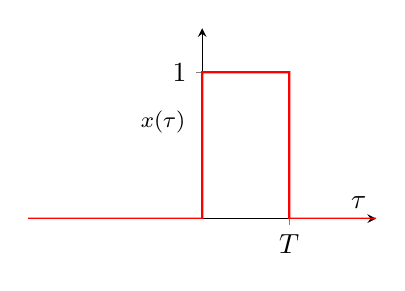
\begin{tikzpicture}
        \begin{axis}[width=6cm,height=4cm,ymin=0,xmin=-2,ymax=1.3,xmax=2, 
                ytick={0,1},
        yticklabels={0,1},
        xtick={1.0},
             xticklabels={$T$},
    xlabel=$\tau$, axis lines = center]

\addplot[color=red,thick] plot coordinates {(-3,0) (0.00001,0) (0.0,1.0) (1.0,1.0) (1.0,0.0) (10,0.0) };
\node at (axis cs:-0.45,0.8) [below, font={\footnotesize}]{$x(\tau)$};

\end{axis}
        \end{tikzpicture}
\end{center}
\caption{Two rectangle functions.}
\label{fig:rectangles}
\end{marginfigure}
An example application of this property is shown in Figure
\ref{fig:sum_lti}. Signals $x_1[n]$ and $x_2[n]$ fed into an identical
LTI systems separately and then added together is equivalent to the
sum of the signals fed into a single LTI system.


\section{Example: Convolution animations}

Animations of the convolution operation for various example systems
can be found here: \url{http://kaira.uit.no/juha/fir_animation/}. The
code for creating such animations can be obtained from GitHub:
\url{https://github.com/jvierine/signal_processing/tree/master/017_fir_animation}.


\section{Example: convolution of two rectangle functions}
Consider the following two continuous-time signals:
\begin{align}
h(t) &= u(t)-u(t-1) \\
x(t) &= u(t)-u(t-T)\,\,.
\end{align}
with $T>1$. These signals are shown in Figure \ref{fig:rectangles}.

The convolution equation includes a term $h(\tau)$ and a term $x(t-\tau)$:
\begin{equation}
y(t)=\int_{-\infty}^{\infty}h(\tau)x(t-\tau)d\tau
\end{equation}
where $x(t-\tau)$ is a time-shifted and time-reversed version of
$x(\tau)$.

The integral can be divided into five different regions with different behaviors.

\noindent \textbf{When $t<0$:}

There is no overlap between $h(\tau)$ and $x(t-\tau)$. The integral is $0$ when $t<0$:
\begin{equation}
y(t) = \int_{-\infty}^{\infty} h(\tau)x(t-\tau)d\tau = 0\,\,.
\end{equation}

\begin{marginfigure}
\if 0
  \begin{center}
        \begin{tikzpicture}
        \begin{axis}[width=7cm,height=3.5cm,ymin=0,xmin=-2,ymax=1.3,xmax=2, 
                ytick={0,1},
        yticklabels={0,1},
        xtick={0.1,1.1},
             xticklabels={$t-T$,$t$},
    xlabel=$\tau$, axis lines = center]

\addplot[color=red,thick] plot coordinates {(-3,0) (0.1,0) (0.1,1) (1.1,1.0) (1.1,0.0) (10,0.0) };

%\addplot[color=red] plot coordinates {(-1,0) (-0.251,0.0) (-0.25,2.0)(0.25,2.0) (0.251,0.0) (1,0)};

\node at (axis cs:0.5,1.0) [below, font={\footnotesize}]{$x(t-\tau)$};

\end{axis}
        \end{tikzpicture}
  \end{center}
  \fi
\begin{center}
        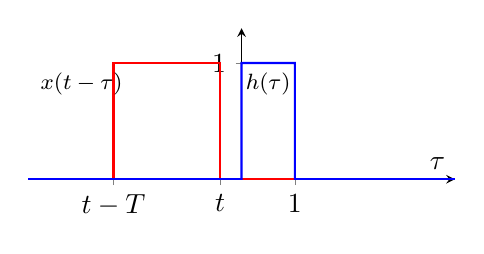
\begin{tikzpicture}
        \begin{axis}[width=7cm,height=3.5cm,ymin=0,xmin=-2,ymax=1.3,xmax=2, 
                ytick={0,1},
        yticklabels={0,1},
        xtick={-1.2,-0.2,0.5},
             xticklabels={$t-T$,$t$,$1$},
    xlabel=$\tau$, axis lines = center]

\addplot[color=red,thick] plot coordinates {(-3,0) (-1.2,0) (-1.2,1) (-0.2,1.0) (-0.2,0.0) (10,0.0) };

\node at (axis cs:-1.5,1.0) [below, font={\footnotesize}]{$x(t-\tau)$};

\addplot[color=blue,thick] plot coordinates {(-3,0) (0.00001,0) (0.0,1.0) (0.5,1.0) (0.5,0.0) (10,0.0) };

\node at (axis cs:0.25,1.0) [below, font={\footnotesize}]{$h(\tau)$};

\end{axis}
        \end{tikzpicture}
\end{center}
\begin{center}
        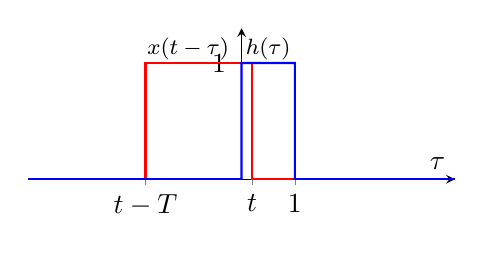
\begin{tikzpicture}
        \begin{axis}[width=7cm,height=3.5cm,ymin=0,xmin=-2,ymax=1.3,xmax=2, 
                ytick={0,1},
        yticklabels={0,1},
        xtick={-0.9,0.1,0.5},
             xticklabels={$t-T$,$t$,$1$},
    xlabel=$\tau$, axis lines = center]

\addplot[color=red,thick] plot coordinates {(-3,0) (-0.9,0) (-0.9,1) (0.1,1.0) (0.1,0.0) (10,0.0) };

\node at (axis cs:-0.5,1.3) [below, font={\footnotesize}]{$x(t-\tau)$};

\addplot[color=blue,thick] plot coordinates {(-3,0) (0.00001,0) (0.0,1.0) (0.5,1.0) (0.5,0.0) (10,0.0) };

\node at (axis cs:0.25,1.3) [below, font={\footnotesize}]{$h(\tau)$};

\end{axis}
        \end{tikzpicture}
\end{center}
\begin{center}
        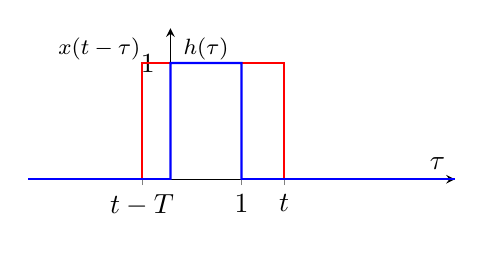
\begin{tikzpicture}
        \begin{axis}[width=7cm,height=3.5cm,ymin=0,xmin=-1,ymax=1.3,xmax=2, 
                ytick={0,1},
        yticklabels={0,1},
        xtick={-0.2,0.8,0.5},
             xticklabels={$t-T$,$t$,$1$},
    xlabel=$\tau$, axis lines = center]

\addplot[color=red,thick] plot coordinates {(-3,0) (-0.2,0) (-0.2,1) (0.8,1.0) (0.8,0.0) (10,0.0) };

\node at (axis cs:-0.5,1.3) [below, font={\footnotesize}]{$x(t-\tau)$};

\addplot[color=blue,thick] plot coordinates {(-3,0) (0.00001,0) (0.0,1.0) (0.5,1.0) (0.5,0.0) (10,0.0) };

\node at (axis cs:0.25,1.3) [below, font={\footnotesize}]{$h(\tau)$};

\end{axis}
        \end{tikzpicture}
\end{center}
\begin{center}
        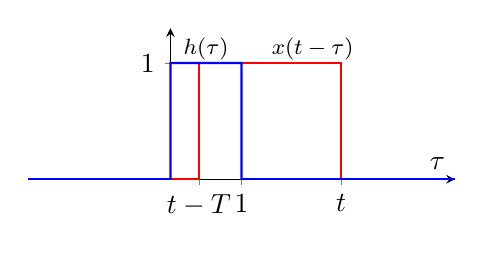
\begin{tikzpicture}
        \begin{axis}[width=7cm,height=3.5cm,ymin=0,xmin=-1,ymax=1.3,xmax=2, 
                ytick={0,1},
        yticklabels={0,1},
        xtick={0.2,1.2,0.5},
             xticklabels={$t-T$,$t$,$1$},
    xlabel=$\tau$, axis lines = center]

\addplot[color=red,thick] plot coordinates {(-3,0) (0.2,0) (0.2,1) (1.2,1.0) (1.2,0.0) (10,0.0) };

\node at (axis cs:1.0,1.3) [below, font={\footnotesize}]{$x(t-\tau)$};

\addplot[color=blue,thick] plot coordinates {(-3,0) (0.00001,0) (0.0,1.0) (0.5,1.0) (0.5,0.0) (10,0.0) };

\node at (axis cs:0.25,1.3) [below, font={\footnotesize}]{$h(\tau)$};

\end{axis}
        \end{tikzpicture}
\end{center}
\begin{center}
        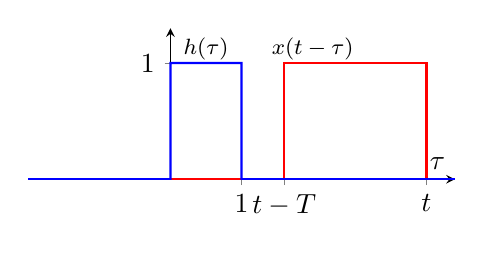
\begin{tikzpicture}
        \begin{axis}[width=7cm,height=3.5cm,ymin=0,xmin=-1,ymax=1.3,xmax=2, 
                ytick={0,1},
        yticklabels={0,1},
        xtick={0.8,1.8,0.5},
             xticklabels={$t-T$,$t$,$1$},
    xlabel=$\tau$, axis lines = center]

\addplot[color=red,thick] plot coordinates {(-3,0) (0.8,0) (0.8,1) (1.8,1.0) (1.8,0.0) (10,0.0) };

\node at (axis cs:1.0,1.3) [below, font={\footnotesize}]{$x(t-\tau)$};

\addplot[color=blue,thick] plot coordinates {(-3,0) (0.00001,0) (0.0,1.0) (0.5,1.0) (0.5,0.0) (10,0.0) };

\node at (axis cs:0.25,1.3) [below, font={\footnotesize}]{$h(\tau)$};

\end{axis}
        \end{tikzpicture}
\end{center}
\caption{Different cases for a convolution of two rectangular functions.}
\label{fig:convolution_example}
\end{marginfigure}

\noindent \textbf{When $0\le t < 1$:}

There is overlap between $h(\tau)$ and $x(t-\tau)$.
\begin{equation}
y(t) = \int_0^{t} d\tau = t\,\,.
\end{equation}

\noindent \textbf{When $1 \le t < T$:}

There is full overlap between $h(\tau)$ and $x(t-\tau)$.
\begin{equation}
y(t) = \int_0^{1} d\tau = 1\,\,.
\end{equation}


\noindent \textbf{When $T \le t \le T+1$:}

There is partial overlap.
\begin{equation}
y(t) = \int_{t-T}^{1}  d\tau = 1-(t-T)\,\,.
\end{equation}


\noindent \textbf{When $t > T+1$:}

There is no overlap.
\begin{equation}
y(t) = 0\,\,.
\end{equation}

\begin{marginfigure}
\begin{center}
        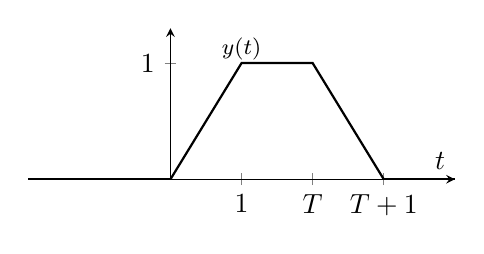
\begin{tikzpicture}
        \begin{axis}[width=7cm,height=3.5cm,ymin=0,xmin=-1,ymax=1.3,xmax=2, 
                ytick={0,1},
        yticklabels={0,1},
        xtick={0.5,1.0,1.5},
             xticklabels={$1$,$T$,$T+1$},
    xlabel=$t$, axis lines = center]


\addplot[color=black,thick] plot coordinates {(-3,0) (0,0) (0.5,1.0) (1.0,1.0) (1.5,0.0) (10,0) };

\node at (axis cs:0.5,1.3) [below, font={\footnotesize}]{$y(t)$};

\end{axis}
        \end{tikzpicture}
\end{center}
\caption{The result of the convolution operation.}
\label{fig:convolution_example2}
\end{marginfigure}

\noindent \textbf{Combined}
\begin{equation*}
y(t) = \left\{ \begin{array}{lcc}
    0 & & t<0  \\
    t & & 0 \le t < 1\\
    1 & & 1 \le t < T\\
    1-(t-T) & & T \le t \le T+1\\
    0 & & t > T+1\\
\end{array}
\right.
\end{equation*}
This is shown in Figure \ref{fig:convolution_example2}.

\section{Applications of convolution}

This chapter only scratches the practical and theoretical uses of
convolution and linear time-invariant systems. I'll use two examples
to illustrate the application of a one dimensional convolution
equation. Be aware that these are by no means the only types of
situations where you will encounter a convolution. Chances are quite
high that a signal processing system you can think of is an LTI
system, or can be approximated as one. Convolution can be found
everywhere!

\subsection{Example: Radar and sonar equation}

\begin{marginfigure}
\begin{center}
\includegraphics[width=\textwidth]{ch10/figures/svalbard.jpg}
\end{center}
\caption{EISCAT Svalbard Radar. The radar echo from the D-region of the ionosphere can be modeled using the equation shown in Equation \ref{eq:convolution_radar}. Photo: Craig Heinselman}
\label{fig:eiscat_svalbard}
\end{marginfigure}
The convolution equation is often used to model radar and sonar
measurements. In this case, the impulse response signal $h[n]$
represents the signal that is scattered as a function of distance. The
signal $x[n]$ represents what a radar or sonar transmits. The signal
received by a radar or sonar receiver $m[n]$ is then modeled as:
\begin{align}
m[n] &=  h[n]*x[n]\\
     &= \sum_{r=0}^{M} h[r] x[n-r]. \label{eq:convolution_radar}\,\,.
\end{align}
In this case, the index $r \in \mathbb{N}$ represents round-trip
propagation time between the transmitter and the receiver. The larger
the distance between the transmitter and the receiver, the larger the
delay. Assuming that the sample rate is $f_s$ in units of hertz or
($\frac{1}{\mathrm{s}}$), and the group velocity of the transmitter
wave $v_g$ ($\frac{\mathrm{m}}{\mathrm{s}}$), the round-trip range is given by:
\begin{equation}
R = \frac{v_g r}{2 f_s}\,\,.
\end{equation}
In the case of radar, the group velocity for electromagnetic waves is
$v_g \approx 3 \cdot 10^8$ ($\frac{\mathrm{m}}{\mathrm{s}}$). For sonar, it is the speed of
acoustic waves within the medium. In the case of air, this is
$v_g \approx 343$ ($\frac{\mathrm{m}}{\mathrm{s}}$).

To see how the convolution equation is the radar equation, we can use
an illustration, as shown in Figure \ref{fig:range_time_diagram}.
\begin{figure}
\begin{center}
\includegraphics[width=\textwidth]{ch10/figures/rd.pdf}
\end{center}
\caption{A range-time diagram depicting the relationship between a transmitted signal and a scattered signal.}
\label{fig:range_time_diagram}
\end{figure}

If the probing signal is a unit impulse $x[n]=\delta[n]$ (a very short
radar pulse), then the measurement directly provides the scattering
amplitude as a function of range:
\begin{align}
m[n] = \sum_{r=0}^M h[r]\delta[n-r] = h[r]\,\,.
\end{align}
This type of radar is called a pulsed radar. In terms of radar
signal processing, this is the easiest case, as no signal processing
is needed! A radar measurement in this case is equivalent to measuring
the ``impulse response'' of the region that the radar is probing.

Here is a fascinating example of a blind child that has learned to
click his tongue (emitting a $\delta[n]$-like impulse sound) to probe the
acoustic scattering of his
surroundings \url{https://www.youtube.com/watch?v=fnH7AIwhpik}. While
this may seem like a superhuman feat, this is not unlike measuring the
distance between yourself and a mountain side by shouting ``echo''
very loudly and counting how long it takes for you to hear a strong
echo. I am sure that many of you have done this already.

If the transmitted waveform $x[n]$ is more complicated than a unit
impulse, the measurements need to be filtered in some way to
reconstruct the scattered signal as a function of range $h[n]$. This
is achieved by designing a filter $\lambda[n]$, which has the
following property $\lambda[n]*x[n] \approx \delta[n]$. After applying
the filter $\lambda[n]$ to the measured signal, one obtains the echo
as a function of range:
\begin{align}
\lambda[n]*m[n] = \lambda[n]*h[n]*x[n] = (\lambda[n]*x[n])*h[n]\approx h[n]\,\,. 
\end{align}
Design of pairs of signals $x[n]$ and filters $\lambda[n]$ is a topic
of radar signal processing. An example of a good pairing of a radar
transmit signal and a receiver filter is shown in the following convolution animation:
\url{http://kaira.uit.no/juha/fir_animation/ex12.gif}.
This is the so-called 13-bit Barker code and the inverse filter that
corresponds to it. The convolution of these two signals is the unit
impulse.


\section{Example: Reverb effect}
\label{reverb_section}

\begin{marginfigure}
\begin{center}
\includegraphics[width=\textwidth]{ch10/figures/mountain_echo.pdf}
\end{center}
\caption{The acoustics of a space are determined by acoustic waves
scattered from various obstacles at various propagation delays. This
can be quite precisely modeled using a convolution, assuming that
nothing is moving.}
\end{marginfigure}
Convolution is encountered when modeling the acoustics of a room or a
space in audio signal processing. The basic underlying principle is
the same as for radar and sonar.

A sound source $x[n]$ is reflected or scattered from different
surfaces within the room at various delays $r$. Each delay $r$
corresponds to the round-trip propagation delay of the acoustic
signal. This is what creates the ``sound'' of a room. This is also
what is the cause for an acoustic ``echo'' from a mountain side that
you may have experienced in real life!

How much signal is scattered from range $r$ is determined by the impulse
response $h[r]$. The resulting signal is a convolution $m[n] = h[n]*
x[n]$. In this case, performing the convolution results in a reverb
effect in acoustic signal processing. 

By accurately modeling the impulse response of a room or a large
concert hall with an impulse response $h[n]$, it is possible to modify
an audio signal $x[n]$ to sound like it was played in that space.

\begin{marginfigure}
\begin{center}
\includegraphics[width=\textwidth]{ch10/figures/reverb.pdf}
\end{center}
\caption{An impulse response that models the acoustics of a large space, with echoes at up to 3 seconds time delay.}
\label{fig:room_model}
\end{marginfigure}


One way to characterize $h[n]$ for a room is to simply measure it. One
emits a very short discrete unit impulse $\delta[n]$ using a high
quality speaker, and then measures the echoes for this pulse to
obtain:
\begin{equation}
h[n] = \sum_{r=0}^M h[r]\delta[n-r]\,\,.
\end{equation}
Another possibility is to model the impulse response $h[n]$ by making
assumptions about the delays of the reflecting surfaces in a room or
space.

The following snippet of code demonstrates modeling of the acoustics
of a room using an modeled impulse response for a room.

\lstinputlisting[language=Python,caption={\texttt{018\_reverb/reverb.py}},label=lst:exercise_reverb]{code/018_reverb/reverb.py}

